\chapter{Introduction and Literature Review} % Chapter Title
\label{LR}

\section{The atmosphere}
\label{LR:Atmos}
  % Overarching description of atmosphere
  The atmosphere is made up of gases held to the earth's surface by gravity. 
  These gases undergo transport on all scales, from barbecue smoke being blown about the garden, to smoke plumes from forest fires travelling across the world and depositing in the Antarctic snow.
  They take part in innumerable chemical reactions along the way, largely driven by solar input and interactions with each other.
  Many gases are lofted into the atmosphere by soil, trees, factories, cars, seas and oceans.
  They are also deposited back to the surface both directly and in rainfall.
  
  % Air
  The atmosphere is made up of nitrogen (N$_2$: $\sim 78\%$), oxygen (O$_2$: $\sim 21\%$), and argon (Ar: $\sim 1\%$), along with water (H$_2$O) and \textit{trace gases} (those that make up less than 1\% of the atmosphere).
  Water (H$_2$O) ranges from $0.001$ to $1\%$ depending on evaporation and precipitation.
  Beyond these major constituents the atmosphere has a vast number of \textit{trace gases}, including carbon dioxide (CO$_2$: $\sim 0.4\%$), Ozone (O$_3$: $.000001$ to $0.001\%$), and methane (CH$_4$: $\sim 0.4\%$) \citep[][Ch. 2]{BrasseurJacob2017}.
  Trace gases in the atmosphere can have a large impact on living conditions.
  They react in complex ways with other elements (anthropogenic and natural), affecting all surface ecosystems upon which life depends.
  
  % TODO: Pressure
  Most of the atmosphere ($\sim 85\%$) is within 10~km of the earth's surface.
  This is due to air pressure, which decreases logarithmically with altitude.
  Any entity is subjected to the weight of all the air above it, and the density of the atmosphere is driven by this pressure.

  % TODO: Structure lead in
  
  \subsection{Structure}
  \label{LR:Atmos:Struct}
    
    The atmosphere extends above us to the edges of space. 
    This is split into various layers, defined by the \textit{lapse rate}: the decrease in temperature with increasing altitude, or $\frac{-\textrm{dT}}{\textrm{dZ}}$.
    Figure \ref{LR:Atmos:Struct:Fig_atmos_layers} shows the pressure and temperature profiles against altitude through the atmosphere.
    The first layer is the troposphere, which extends to roughly 10~km and is characterised by positive lapse rate (or decreasing temperature with altitude).
    At the top of the troposphere (the tropopause) the temperature stops decreasing, and then the stratosphere is defined by a negative lapse rate.
    This is due to UV radiation being absorbed by ozone, and leads to a very vertically stable environment.
    
    \begin{figure}
      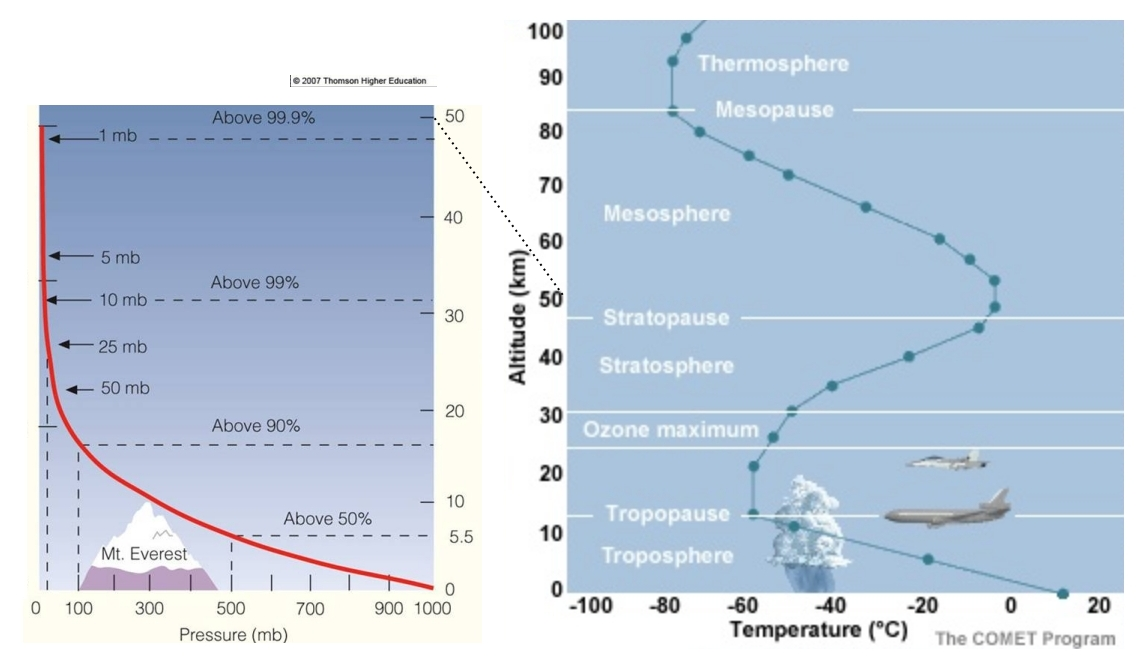
\includegraphics[width=\textwidth]{Figures/Atmos_Temp_Press.jpg}
      \caption{%
        Pressure (red) logarithmically decreasing, shown with percentage of atmosphere below at several points.
        Temperature (green) changes throughout the atmosphere.
        Figure edited from \url{https://climate.ncsu.edu/edu/Structure}.
      }
      \label{LR:Atmos:Struct:Fig_atmos_layers}
    \end{figure}
    
    
    
    % Boundary layer
    In addition to these atmospheric layers, the troposphere can be subset: into a \textit{boundary layer}, and the \textit{free troposphere}.
    The \textit{boundary layer} is the lowest layer and involves increased atmospheric mixing due to ground heating and friction effects.
    It generally extends anywhere from 200 - 1000~m, above which the ground effects have fewer direct impacts.
    The \textit{free troposphere} is the remainder of the troposphere and is more affected by transport, both horizontally and from the stratosphere.
    
    
  % Chemistry
  \subsection{Composition}
  \label{LR:Atmos:Chem}
    %TODO: Overviewish paragraph
    TODO overview here
    Oxidation and photolysis are the two main processes whereby compounds are broken down in the atmosphere.
    
    % Oxidation and Radicals
    \subsubsection{Hydroxyl radicals}
    %\label{LR:Atmos:Chem:radicals}
      OH and HO$_2$ concentrations largely determine the oxidative capacity of the atmosphere.
      The OH radical drives many processes in the atmosphere, especially during the day when photolysis of ozone drives OH concentrations \citep{Atkinson2000}.
      OH is a key species which reacts with nearly all the organic compounds in the troposphere, with only a few exceptions \citep{Atkinson2000}.
      %The exceptions are chlorofluorocarbons (CFCs), and Halons not containing H atoms \citep{Atkinson2000}.
      Over land, isoprene (C$_5$H$_8$) and monoterpenes (C$_{10}$H$_{16}$) account for 50\% and 30\% of the OH reactivity (defined in section TODO) respectively \citep{Fuentes2000}. %TODO add OH reactivity definition to modelling chapter
      
      Since radicals are involved in all oxidative chemistry in the atmosphere it is important for models to accurately represent them (eg. \cite{Travis2014}).
      This is difficult as they are coupled with so many other species and measurements of OH are not readily available on a global scale.
      In the late 90's it was thought that OH radicals were formed exclusively from photolysis of O$_3$, HONO, HCHO, and other carbonyls (R$_2$C=O) \cite{Atkinson2000}.
      It has been shown since that TODO. %TODO more on OH sources
      Isoprene (C$_5$H$_8$) was thought to be a sink of OH until it was shown by \cite{Paulot2009b} that the radicals are recycled.
      This recycling process is discussed in more detail in section \ref{LR:VOCs:IsopCascade}.
      
      Ozone is an important precursor to OH, as excited oxygen atoms (O(${}^1$D) are created through its photolysis, which then go on to react with water to form OH, as shown in this reaction sequence \citep{Atkinson2000, AtkinsonArey2003}:
      \begin{equation}
      \begin{aligned}
      O_3 + \text{hv}         & \to  O_2 + O({}^1D)   && (\lambda \le 350 \text{nm}) \\%
      O({}^1D) + M            & \to  O({}^3P) + M     && (M=N_2, O_2)               \\%
      O({}^3P) + O_2 + M      & \to  O_3 + M          &&                           \\%
      O({}^1D) + H_2O         & \to  2OH              &&                            \\%
      \end{aligned}
      \label{LR:Atmos:Chem:eqn_O3toOH}
      \end{equation}
      This shows that some of the O$({}^1D)$ recycles back to ozone, while some forms OH.
      \cite{AtkinsonArey2003} discuss the relative rates of these reactions.

\section{Ozone}
\label{LR:O3}
  %TODO What is ozone
  
  %Structure of ozone layer chapman eqn etc.
  Ozone (O$_3$) is mostly located in the stratosphere, where it helpfully prevents much of the shorter wave length solar radiation from reaching the earth's surface (ie UV light).
  In the stratosphere ozone production is generally driven by the Chapman mechanism, as high energy light (with wavelengths $\lambda<242$~nm) photolyses the molecular oxygen (O$_2$) in the atmosphere \citep[][Chapter 3, section 2]{BrasseurJacob2017}.
  
  The Chapman mechanism involves several equations which lead to rough equilibrium of O, O$_2$, O$_3$ and pressure, as follows:
  \begin{equation}
  \begin{aligned}
  \textrm{O}_2 + hv(\lambda < 242 \text{nm}) & \rightarrow & \text{O} + \text{O} \\
  \text{O} + \text{O}_2 + \text{M} & \rightarrow & \text{O}_3 + \text{M} \\
  \text{O}_3 + hv(\lambda < 1180 \text{nm}) & \rightarrow & \text{O} + \text{O}_2 \\
  \text{O} + \text{O}_3 & \rightarrow & \text{O}_2 + \text{O}_2 \\
  \end{aligned}
  \label{LR:O3:eqn_Chapman}
  \end{equation}
  Where $hv$ represents radiation and M is an inert molecule (such as N$_2$).
  The high energy photons ($\lambda < 242$~nm) are present from the top of the atmosphere but are mostly removed before reaching the troposphere.
  The lifetime of O against loss by O$_2$ is less than a second in the troposphere, and produced O$_3$ quickly returns to O and O$_2$, as low energy ($\lambda < 1180$~nm) light and M are abundant.
  The gradient of light penetration in addition to the logarithmic decrease in atmospheric pressure (which affects M abundance) drives the vertical profile of ozone into what is called the ozone layer, where we have relative abundance of ozone in the stratosphere.
  This mechanism requires radiation so only takes place during the daytime, during the night there are different processes driving ozone chemistry.
  
  Ozone in the lower atmosphere is a serious hazard that causes health problems \citep{Hsieh2013}, damages agricultural crops worth billions of dollars \citep{Avnery2011,Yue2017}, and increases the rate of climate warming \citep{IPCC_2013_chap8}.
  Around 5 to 20 percent of all air pollution related deaths are due to ozone (\cite{Monks2015}), roughly .8 million deaths per year (\cite{Lelieveld2013}).
  In the short term, ozone concentrations of $\sim$50-60~ppbv over eight hours or $\sim$80~ppbv over one hour are agreed to constitute a human health hazard \citep{Ayers2006,Lelieveld2009}. 
  Long term exposure causes problems with crop loss and ecosystem damage \citep{Emberson2003}, and worryingly, concentrations may get worse in the future \citep{Lelieveld2009, Stevenson2013}.
  Further tropospheric ozone enhancements are projected to drive reductions in global crop yields equivalent to losses of up to \$USD$_{2000}$ 35 billion per year by 2030 \citep{Avnery2011}, along with detrimental health outcomes equivalent to $\sim$\$USD$_{2000}$11.8 billion per year by 2050 \citep{Selin2009}.
  Recently \cite{Yue2017} showed that the net effect of near-surface ozone on is a $\sim 14\%$ decrease in net primary productivity (NPP) in China.
  They state that drastic measures could reduce the decrease by $\sim 70\%$ by 2030.
  
  % Measurements
  Since the Montreal Protocol on Substances that Deplete the Ozone Layer was established in August 1987, and ratified in August 1989, several satellites and many measurement stations were set up to monitor ozone in the stratosphere.
  However, in the southern hemisphere there are relatively few records of ozone (\cite{Huang2017}).
  This affects our ability to accurately determine sources of ozone in the troposphere.
  
  % Models
  Models of ozone in the atmosphere are used broadly for international assessments of ozone related emissions \citep{Young2018}.
  \cite{Young2018} summarise current global ozone modelling standards and the metrics and processes used to evaluate these models.
  They show how models can be used to improve measurements, estimate concentrations in regions not sampled, and allow analysis of other processes which involve ozone (such as radiation).
  
  %What drives ozone in the troposphere? 
  Generally there are two main drivers of tropospheric ozone concentrations; transport from the stratosphere and production due to emissions of precursors. 
  Globally, most tropospheric ozone is produced by naturally emitted (biogenic) precursors.
  At small to medium scales, pyrogenic (fire) and anthropogenic (man-made) emissions can be important.
  Smoke plumes from biomass burning can carry ozone precursors, creating higher ozone concentrations downwind of the plume's source.
  Emissions of precursors from large cities (such as NO$_X$ emissions from traffic and power production) can impact ozone concentrations.
  
  A good summary of processes affecting tropospheric ozone, copied from \cite{Young2018}, is shown in Figure \ref{LR:O3:YoungOzoneSummary}.
  This picture shows the major processes used by global chemistry models when simulating tropospheric ozone.
  In each gridbox both physical and chemical processes need to be accounted for.
  
  \begin{figure}
    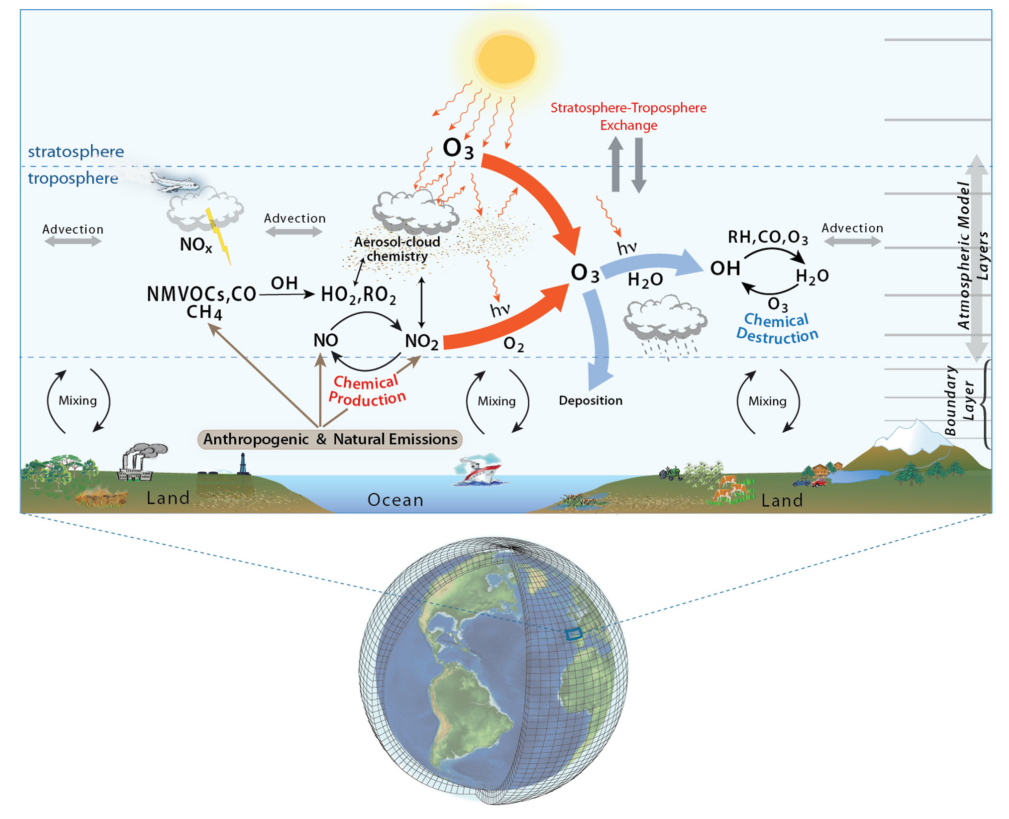
\includegraphics[width=\textwidth]{Figures/Young2018_Figure1.png}
    \caption{%
      Tropospheric ozone processes, Figure 1 in \cite{Young2018}.
      DOI: https://doi.org/10.1525/elementa.265.f1
      }
    \label{LR:O3:YoungOzoneSummary}
  \end{figure}
  
  \subsubsection{NOx}
  NO$_X$ ($\equiv $ NO$_2$ and NO) is another important chemical family in the atmosphere which interacts with ozone and regulates the atmospheric oxidative capacity.
  NO$_X$ is a short lived compound, with emissions (Power generation and combustion transport) the main driver of its' concentration \citep{Delmas1997}.
  %TODO cite
  When NO$_X$ and O$_3$ relative concentrations during the day are regulated by the following reactions \citep{Atkinson2000}:
  \begin{equation}
  \begin{aligned}
  NO + O_3         & \to NO_2 + O_2      && \\%
  NO_2 + O_3       & \to NO_3 + O_2      && \\%
  NO_3 + \text{hv} & \to NO + O_2        && (\sim 10\%)  \\%
  NO_3 + \text{hv} & \to NO_2 + O({}^3P) && (\sim 90\%)  \\%
  \end{aligned}
  \label{LR:Atmos:Chem:eqn_O3toNO2}
  \end{equation}
  Which generally leads to lower ozone concentrations in cities due to the NO$_X$ pollution.
  
  \subsection{Stratosphere to troposphere transport}
    \label{LR:O3:STT}
    %% STT
    Historically (in the late 1990's), ozone transported down from the stratosphere was thought to contribute 10-40~ppb to tropospheric ozone levels, matching tropospheric production \citep{Atkinson2000, Stohl2003}.
    This number was revised down over the years as measurement and modelling campaigns improved our understanding of global scale transport, mixing, and chemistry \citep{Monks2015}.
    Recently \cite{Kuang2017} analysed various measurements in south-east USA and observed STT influence which can be seen to affect surface ozone levels.
    In their work they use various measurements from different instruments to give the structure and temporal evolution of ozone and the local weather system.
    
    Ozone transported to the troposphere from the stratosphere can occur through diffusion (relatively slowly), or direct mixing.
    Intrusions of stratospheric air into the troposphere are often called Stratosphere to Troposphere Transport events (STT).
    STT often occur as tongues of stratospheric air descend and get disconnected from the stratosphere, potentially due to low pressure systems and jet streams \cite{Sprenger2003}.
    Recently global chemical transport models (CTMs) have been used to trace how much ozone is being transported to the troposphere from the stratosphere.
    There are a few methods of doing this, such as \cite{Ojha2016}, who use the ECHAM5 CTM with a tracer that keeps track of ozone formed and transported from the stratosphere.
    Model based estimates generally require validation against actual measurements, such as those from ozonesondes or satellites.
    %Hegglin, M. I., and T. G. Shepherd (2009), Large climate-induced changes in ultraviolet index and stratosphere-to-troposphere ozone flux, Nature Geosci, 2(10), 687 \selectlanguage{english}691, doi:10.1038/NGEO604.
    \cite{Hegglin2009} estimate that climate change will lead to increased STT due to an acceleration in the Brewer Dobson circulation.
    They estimate $\sim 30$, and $\sim 121$~Tg yr$^{-1}$ increases (relative to 1965) in the southern and northern hemispheres respectively
    
    \cite{Liu2017} examine southern hemispheric ozone and the processes which control its inter-annual variability (IAV).
    IAV is the standard deviation of ozone anomalies from the monthly mean.
    They show that ozone transported from the stratosphere plays a major role in the upper troposphere, especially over the southern Indian ocean during austral winter.
    While stratospheric transport mostly impacts the upper troposphere, some areas are impacted right down to the surface.
    \cite{Liu2017} look at modelled tropospheric ozone sensitivity to changes in stratospheric ozone, ozone precursor emissions, and lightning over the southern hemisphere from 1992--2011. 
    Their work suggest ozone at 430~hPa is mostly stratospheric in September over 20$^{\circ}$S to 60$^{\circ}$S at all longitudes.
    They also see tropospheric ozone sensitivity to emissions from South America (0--20$^{\circ}$S, 72.5--37.5$^{\circ}$W), southern Africa (5--10$^{\circ}$S, 12-38$^{\circ}$E), and South to South-east Asia (70-125$^{\circ}$E, 10$^{\circ}$S--40$^{\circ}$N).
    In the USA recent work by \cite{Lin2015} suggests that intrusions during spring are increasing surface ozone levels.
    Their work also recommends that understanding of frequency and cause of STT needs to be improved to effectively implement air quality standards.
    
    
  
  \subsection{Chemical production}
    An analysis of the Atmospheric Chemistry and Climate Model Inter-comparison Project (ACCMIP) simulations by \cite{Young2013} found STT is responsible for $540\pm140$~Tg yr$^{-1}$, equivalent to $\sim$11\% of the tropospheric ozone column, with the remainder produced photochemically \citep{Monks2015}.
    A recent summary by \cite{Young2018} estimates ozone production and loss in the troposphere to be $\sim$4900\tgpyr, and $\sim$4500\tgpyr respectively, while STT sources are $\sim$500\tgpyr. 
    They also show how all these figures are still relatively uncertain.
    
    tropospheric ozone concentrations rely on climate and ozone precursor emissions; including NO, NO$_2$, CO, VOCs, and HCHO \citep{Atkinson2000, Young2013, Marvin2017}. 
    Ozone predictions are uncertain due to the vagaries of changing climate which affects both transport, deposition, destruction, and plant based precursor emissions.
    All of these processes are tightly coupled and difficult to accurately model, as they depend on uncertain assumptions such as CO$_2$ dependency \citep{Young2013}.
    Even with all the work done over the prior decades there remains large uncertainties about ozone precursors in the troposphere \citep{Mazzuca2016}.
    
    %% How VOCs and Ozone interact:
    Ozone is formed in the troposphere through oxidation of VOCs (described in Section \ref{LR:VOCs})) in the presence of NO$_X$.
    Net formation or loss of O$_3$ is determined by interactions between VOCs, NO$_X$, and HO$_X$, and is a complicated system of positive and negative feedbacks \citep{Atkinson2000}.
    Figure \ref{LR:VOCs:fig_NOXVOCOzone} shows the non-linear affect of NO$_X$ and VOC concentrations on ozone production over Houston, as modelled in \cite{Mazzuca2016}.
    Recently the relationship has been examined on the intradiel timescale showing that ozone production can be more or less sensitive to VOCs at different hours depending on location various other factors \citep{Mazzuca2016}.
    
    \begin{figure}
      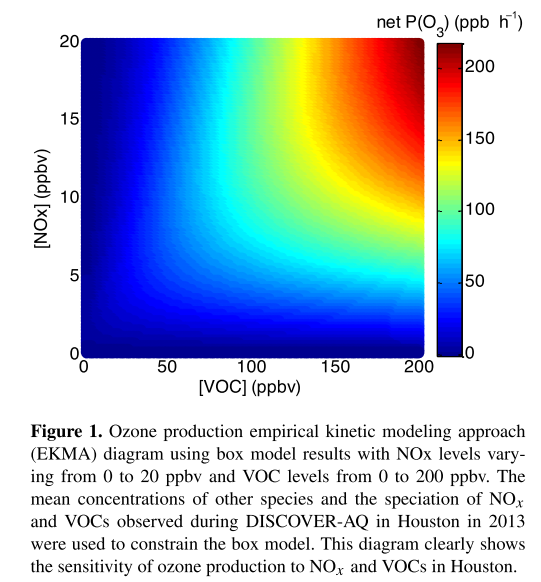
\includegraphics[width=.75\textwidth]{Figures/Mazzuca2016_NOxVOCOzone.png}
      \caption{Ozone production figure copied from \cite{Mazzuca2016}.}
      \label{LR:VOCs:fig_NOXVOCOzone}
    \end{figure}
    
    
    %TODO: formulae which regulate ozone levels 
    Ozone in rural areas is often higher than in populous cities, as the high NO levels titrate the O$_3$.
    Equation \ref{LR:Atmos:Chem:eqn_O3toNO2} shows how NO and O$_3$ lead to NO$_2$ and the very short lived NO$_3$ radical.
    
    % Loss pathways
    Tropospheric ozone is lost via chemical destruction and dry deposition, estimated to be $4700\pm700$ Tg yr$^{-1}$ and $1000\pm200$ Tg yr$^{-1}$, respectively \citep{Stevenson2006,Young2018}.
    The main loss channel is through equation \ref{LR:Atmos:Chem:eqn_O3toOH}, where photolysis and pressure create OH from the O$_3$.
    

\section{VOCs}
\label{LR:VOCs}
  % What they are
  Organic compounds are members of a large class of chemicals whose molecules contain carbon, with the exception of a few compounds such as carbides, carbonates (CO$_3$), and simple oxides of carbon and cyanides.
  Organic compounds can be categorised based on their vapour pressure, which is the tendency of a liquid or solid to vaporise.
  Compounds with high vapour pressures at standard temperature are classed as volatile, and have a felicity to evaporate at low temperatures.
  Plants contain tens of thousands of organic compounds, it's likely that fewer than 40 are emitted due to the low volatility of most of them \citep{Guenther2000}.
  
  Atmospheric organic compounds are legion and differ by orders of magnitude with respect to their fundamental properties, such as volatility, reactivity, and cloud droplet formation propensity, etc.
  Volatile organic compounds (VOCs) have vapour pressure greater than $10^{-5}$~atm, and are mostly generated naturally by plants, which emit around 1000\tgpyr \citep{Guenther1995, Glasius2016}.
  Due to their high volatility these compounds are generally seen in the gas phase.
  Organic compounds with a lower volatility are classed as semi-volatile (SVOCs: vapour pressure between $10^{-5}$ and $10^{-11}$~atm) are seen in both gas and particle phase depending on temperature and pressure.
  Organic compounds with even lower vapour pressure are generally found in the particle phase in aerosol particulate matter \citep{Glasius2016}.
  Understanding the drivers of trends in biogenic VOC emissions (BVOCs) is needed in order to estimate future carbon fluxes, changes in the water cycle, air quality, and other climate responses \citep{Yue2015}.
  In the last 20 years anthropogenic emissions of VOCs have been increasing while biogenic VOC emissions have decreased, due to rapid economic growth and lower annual temperatures \citep{Stavrakou2014, Kwon2017}.
  

  %% What do VOCs do?
  VOCs are an important driver of atmospheric processes, especially near forests.
  VOCs are broken down into HCHO, O$_3$, CO$_2$ and various other species, mainly through oxidation (by OH).
  VOC emissions result in radical cycling, acid deposition, production of tropospheric ozone, and secondary organic aerosols (SOAs) \citep{Atkinson2000, Kanakidou2005}.
  A regional-model study in Europe (\cite{Aksoyoglu2017}) has also shown VOCs impact secondary inorganic aerosol concentrations.
  These have impacts on climate (through radiative forcing) and air quality, affecting both human health and crop yields \citep{IPCC_Chapter2, Avnery2011, Lelieveld2015}.
  
  % voc sources
  The major source of VOCs in the atmosphere is biogenic, with around 90\% of emissions (globally) coming from natural sources \citep{Guenther1995,Guenther2006, Millet2006}.
  Methane (CH$_4$) is one of the more abundant and potent VOCs, however it is often classified separately and compared against non-methane VOCs (NMVOCs).
  NMVOCs are alkanes, alkenes, aromatic hydrocarbons and isoprene, with isoprene being the most prominent.
  Methane and isoprene each comprise around a third of the global total emissions of VOCs (\cite{Guenther2006}).
  However, methane is relatively long lived (years) and is well mixed in the atmosphere while isoprene levels are very volatile and spatially diverse due to a life time of around an hour.
  In this thesis I work towards a better understanding of the NMVOC emissions coming from Australia.
  
  % voc removals
  VOCs are removed by wet and dry deposition, OH oxidation, reaction with NO$_3$, ozonolysis (at night time or in polluted areas) or photolysis \citep{AtkinsonArey2003, Brown2009}.
  The process of deposition only accounts for a small fraction of the VOC loss, with the possible exception of the long lived methane compound \citep{AtkinsonArey2003}.
  
  %%% PM and SOA
  PM in the atmosphere is a major problem, causing an estimated 2-3 million deaths annually \citep{Hoek2013, Krewski2009, Silva2013, Lelieveld2015}. 
  Aerosols are suspended particulates and liquid compounds in the atmosphere, of which particulate matter (PM) is an important subset.
  Fine particulate matter (PM$_{2.5}$) penetrates deep into the lungs and is detrimental to human health.
  Some PM comes from small organic aerosols (OA) emitted in the particulate phase and referred to as primary OA (POA).
  A substantial amount of PM is due to gaseous organic compounds transforming in the troposphere leading to what's known as secondary OA (SOA) \citep{Kroll2008}.
  
  Formation of SOA is generally due to VOC oxidation and subsequent reactions, while removal from the atmosphere is largely due to wet or dry deposition, and cloud scavenging \citep{Kanakidou2005}.
  It can be difficult to attribute PM formation, in part due to the complex relationship between NO$_X$, OH, O$_3$, and the uncertainty surrounding precursor emissions.
  Improved concentration estimates of these organic compounds requires a better understanding of their emissions, which is one of the foci in this thesis.
  
  \subsection{Isoprene}
  \label{LR:VOCs:Isop}
    Isoprene, or 2-methylbuta-1,3-diene, is a VOC with the chemical formula C$_5$H$_8$. 
    It is of major importance to the atmosphere, as it is involved in various processes which alter the oxidative capacity of the atmosphere.
    \cite{Guenther1995}, and subsequent updates \citep{Guenther2000,Guenther2006,Guenther2012}, have been used ubiquitously by the atmospheric community as a global estimate of isoprene emissions, at roughly 500-600\tgpyr, emitted mostly during the day.
    Recently an estimate of global isoprene emissions has been made using a completely different model, of around 465~Tg C yr$^{-1}$, by \cite{Messina2016} using ORCHIDEE.
    The global emission factors model used to derive both these estimates is based on modelling emissions from different plant species (phenotypes), and relatively few Australian species are used when forming in these estimates.
    
    Isoprene affects NO$_X$ and HO$_Y$ cycling, see for example formulae \ref{LR:Atmos:Chem:eqn_O3toOH}, \ref{LR:Atmos:Chem:eqn_O3toNO2}.
    In the presence of NO$_X$, isoprene forms tropospheric ozone and SOAs \citep{Wagner2002, Millet2006}.
    It has a short lifetime during the day, roughly an hour due to OH oxidation \citep{AtkinsonArey2003}).
    
    
    %% HOW its measured:
    Measurements of isoprene are often uncertain or difficult to make accurately.
    \cite{Kanakidou2005} summarised how chamber experiments used to measure isoprene reactions may be unsuitable for comparison to the natural atmosphere.
    In \cite{Nguyen2014} many scientists and groups worked together on chamber measurements, to improve understanding of ambient atmospheric oxidation mechanisms of biogenic hydrocarbons (such as isoprene).
    %% CHAMBER study examples?
    
    
  \subsection{Emissions}
  \label{LR:VOCs:Emissions}
    
    
    Isoprene emissions are often classified as either anthropogenic, biogenic, or pyrogenic.
    The natural or biogenic sources are roughly ten times higher than the anthropogenic VOC sources \citep{Guenther2006, Kanakidou2005}.
    Major emitters are tropical broadleafs (notably eucalypts), and scrubs \citep{Guenther2006, Arneth2008, Niinemets2010, Monks2015}.
    TODO: why do plants emit?
    Emissions are affected by various factors such as temperature, sunlight, soil moisture, etc.
    
    It used to be thought that emissions of anthropogenic and biogenic VOCs (AVOCs, BVOCs respectively) were roughly similar (\cite{Muller1992}, TODO: more cites).
    In the 1990's it became clear that biogenic emissions of VOCs were in fact dominant, although methane emissions are still largely anthropogenic. 
    Global NMVOC levels are estimated at 85~\%, 13~\%, and 3~\% from biogenic, anthropogenic, and pyrogenic sources respectively \citep{Kanakidou2005, Kefauver2014}.
    
    The World Meteorological Organisation (WMO) estimated that we are emitting 360~Mt yr$^{-1}$ of methane, compared to biogenic emissions of around 200~Mt yr$^{-1}$ \citep{Atkinson2000}.
    In 1995 emissions of other VOCs were estimated at 1150\tgcpyr from biogenic sources, and 100\tgcpyr from anthropogenic sources \citep{Guenther1995, Atkinson2000}.
    The main non-methane BVOC emissions are isoprene (44\%) and monoterpenes (11\%) (\cite{Guenther2000, Kefauver2014}). 
    Land use changes can drastically affect isoprene sources, for instance in the tropics where large scale deforestation has converted forest into crop lands \citep{Kanakidou2005}.

    Biogenic VOC emissions affect surface pollution levels, potentially enhancing particulate matter (PM) and ozone levels.
    
    
    % Lead in to isoprene cascade
    Isoprene is emitted and enters the atmosphere in the gas phase, where it reacts with various chemicals, forming many new chemicals with reactions at various time scales.
    One common compound which is produced by these reactions is HCHO, which is easier to measure and often used to estimate how much isoprene is being emitted.
    There are many reactions which occur and are important to capture in models due to their impacts on air quality and physical properties in the lower atmosphere.
    The many children processes and products which begin with isoprene oxidation are often called the isoprene (photochemical) cascade \cite{Crounse2012,Paulot2012,Wolfe2016}.
    
  \subsection{The isoprene cascade}
    \label{LR:VOCs:IsopCascade}
    %TODO: Isoprene cascade reordering !
    % TODO: Find nice picture of isoprene products up to 2nd gen + yields if possible
    
    Isoprene forms many products with various lifetimes, here I will present an overview of some important mechanisms and products which are useful to my work.
    
    Photolysis and oxidation of many VOCs initially form alkyl radicals ($\dot{R}$).
    Alkenes (VOCs with double bonded carbon, such as isoprene) react with ozone leading to organic peroxy radicals (RO$\dot{O}$). 
    These go on to form many products and lead to (amongst other things) aerosol, formaldehyde, and ozone formation, depending on various other factors such as sunlight and NO pollution \citep{Atkinson2000}.
    
    \subsubsection{Oxidation}
    The primary first step for atmospheric isoprene is photooxidation, reacting with OH to form isoprene hydroxyperoxy radicals (\roo) (\cite{Wolfe2016,Marvin2017,Patchen2017}).
    There is still uncertainty about which pathways are most important following \roo production: HO$_2$ reactions predominantly produce hydroxyhydroperoxides (ISOPOOH), NO reactions largely produce methyl vinyl ketone (MVK) and methacrolein (MCR), and RO$_2$ reactions are also possible \cite{Liu2016a}.
    
    
    The first step in oxidising alkenes (including isoprene) is a replacement by OH of a double bond, as summarised by the equation from \cite{Patchen2007}:
    % Uses package{mchem}
    \ce{R-CH=CH-R$^{\prime}$ + OH -> R-CH(OH)CH-R$^{\prime}$ }
    where R and R$^{\prime}$ represent hydrocarbons.
    This OH adduct then reacts with O$_2$ to produce a hydroxyperoxy radical (\roo), which for isoprene can be any of six different isomers \citep{Patchen2007}.
    These \roo (also called organic-peroxy/alkyl-peroxyl/ISOPOO radicals, or RO$_2$)  react with HO$_2$ or NO and produce stable products (often called oxidised VOCs or OVOCs) \citep{Nguyen2014}.
    The \roo react with various compounds including NO, HO$_2$ and other \roo, with most pathways potentially producing HCHO \citep{Wolfe2016}.
    
    
    This is where the isoprene oxidation path splits depending on the NO$_X$ concentration.
    Reactions with NO can lead to ozone production in environments rich in isoprene or other non-methane organic compounds (NMOCs) and NMVOCs (\cite{Patchen2007,AtkinsonArey2003}).
    These reactions are complex and coupled, for example NO$_2$ concentrations can be increased by NMOC and NO reactions \citep{AtkinsonArey2003}.
    In the presence of NO$_X$, the \roo may form organic nitrates after reacting with NO.
    Any organic nitrates which are formed affect levels of both HO$_X$ (H, OH, peroxy radicals) and NO$_X$, acting as a sink (\cite{Mao2013} and references therein).
    
    %% NO2 reaction -> nitrates
    Reaction with NO$_2$ forms isoprene nitrates, or hydroxynitrate (RONO$_2$).
    The first generation of organic nitrates produced by isoprene oxidation range from 7\% to 12\%, shown in laboratory experiments \citep{Paulot2009a, Mao2013},
    A portion of isoprene nitrates are recycled back to NO$_X$, so may serve as a reservoir of nitrogen and allow its transport to the boundary layer of remote regions (\cite{Patchen2007,Paulot2009a}).
    The nitrates can also build up in the winter, when removal processes are not as dominant \citep{Lelieveld2009}.
    % Nox paragraph?
    NO$_X$ is removed primarily by conversion to nitric acid (HNO$_3$) followed by wet or dry deposition \citep{Ayers2006}.
    
    Oxidation reactions are important and quickly stabilise the ratio of NO to NO$_2$. 
    There is still large uncertainty around the fate of various \roo, which limits understanding of the relative importance of some chemical processes \citep{Crounse2013}.
    
    Some portion of emitted isoprene leads to SOA, potentially through the formation of methacrylic acid epoxide (MAE) formed by decomposition of methacryloylperoxynitrate (MPAN, a second generation product of isoprene oxidation) as shown in smog chambers and field studies in \cite{Lin2013}.
    
    %% LOW NOX scenario
    Isoprene oxidation by OH is less well understood when lower concentrations of NO are present in the atmosphere.
    Initially isoprene was thought to be a sink for atmospheric oxidants \citep[e.g.][]{Guenther2000}.
    It was thought that in low NO environments, like those far from anthropogenic pollution and fires, oxidation of isoprene would create ISOPOOH and lead to low concentrations of OH and HO$_2$ \cite{Paulot2009b}.
    In \cite{Paulot2009b}, the HO$_X$ levels are shown to be largely unaffected by isoprene concentrations.
    They show that ISOPOOH is formed in yields $> 70\%$, and MACR and MVK is formed with yields $< 30\%$.
    The formation of MACR and MVK produces some HO$_X$, although not enough to close the gap.
    \cite{Paulot2009b} goes on to suggest (and provide experimental evidence) that dihydroxyperoxides (IEPOX) are formed from oxidation of the ISOPOOH, which form precursors for SOAs as well as closing the HO$_X$ concentration gap.
    They then use GEOS-Chem, modified to include IEPOX formation, to estimate that one third of isoprene peroxy radicals react with HO$_2$, and two thirds react with NO. 
    They estimated $95 \pm 45$\tgpyr IEPOX being created in the atmosphere, which (at the time) was not modelled by CTMs.
    Their work showed another pathway for isoprene based SOA creation, through these IEPOX creation and HO$_X$ recycling mechanisms.
    \cite{Peeters2010} suggested that the work of \cite{Paulot2009b} only partially bridges the gap between clean air OH concentration measurements and models.
    They suggested four new mechanisms for OH recycling in these pristine conditions.
    These can be summarised as OH regenerating reactions which occur during photolysis of hydroperoxy-methyl-butenals (HPALDs), and resulting photolabile peroxy-acid-aldehydes (PACALDs).
    These reactions are highly non-linear and subject to large uncertainty, however when compared against several campaigns they were shown to improve one particular models (IMAGES) HO$_X$ concentrations.
    In \cite{Crounse2012}, MACR products are examined in various conditions and hydroxy recycling is also observed in low NO conditions.
    
    Although understanding of OH production/recycling in these low NO conditions has been improved, many observations of OH were still quite under-predicted in models \citep{Mao2012}.
    \cite{Mao2012} showed how traditional OH measurements may be overestimated due to VOC oxidation.
    They looked at measurements in a remote forest in California and found that the instruments were generating OH internally.
    \cite{Nguyen2014} also see this VOC oxidation interference in measurements using a gas chromatographer (GC) with an equipped flame ionisation detector (FID).
    This lends more credence to the current understanding of VOC oxidation as it closed the gap between measurements and model predictions (\cite{Mao2012}).
    
    \cite{Peeters2010} showed that HO$_2$ is produced at near unity yields following isoprene oxidation initiated by OH.
    TODO: read more Peeters2010
    
    \cite{Nguyen2014} examine various measurement techniques to determine isoprene reactions in non-laboratory conditions.
    Their work discussed how large uncertainties persist in isoprene oxidation, which carries through to predictions by atmospheric models.
    \cite{Nguyen2014} show preliminary estimates of low-NO yields of MVK and MCR to be 6$\pm3\%$ and 4$\pm2\%$ respectively, consistent with TODO:\cite{Liu2013}, but only when cold-trapping methods are employed.
    These yields each increase (due to interference by OVOCs) to greater than 40\% when directly sampled by GC-FID.
    
    Even with the recent boom in isoprene analysis, uncertainties remain in the isoprene oxidation mechanisms.
    Examples (taken from \cite{Nguyen2014}) include isoprene nitrate yields, which range from 4-15\% \citep{Paulot2009a}, 90\% disagreements in MAC and MVK yields TODO:\citep{Liu2013}, various possible sources for SOA TODO:\citep{Chan2010, Surratt2010, Lin2013}, unknown HPALD fates, incomplete O$_2$ incorporation TODO:\citep{Peeters2009,Crounse2013}, and under-characterized RO$_2$ lifetime impacts TODO:\citep{Wolfe2012}. TODO: get those citations and read abstracts.
    
    \subsubsection{Ozononlysis}
    Ozononlysis is the splitting of carbon chains by ozone molecules, and is among the primary oxidation pathway for volatile alkenes \citep{Nguyen2016}.
    Criegee intermediates (carbonyl oxides with two charge centres) are formed when isoprene reacts with O$_3$. 
    \cite{Nguyen2016} examine in detail a few of these, with proposed mechanisms for C$_1$ and C$_4$ Criegee intermediate reactions.
    The C$_1$ stabilised Criegee (CH$_2$OO, $\sim 61\%$) is therein proposed to react with water yielding $73\%$ hydroxymethyl hydroperoxide (HMHP), $6\%$ HCHO $+$ H$_2$O$_2$, and formic acid $+$ H$_2$O, and the same products with yields of 40, 6, and 54$\%$ respectively when this Criegee reacts with (H$_2$O)$_2$.
    TODO: more on Nguyen2016?
    
    \subsubsection{Oxidation by NO3}
    At night when OH concentrations have dropped, isoprene can remain in the atmosphere to be transported.
    Typically less than half of this night time isoprene is removed through ozonolysis \citep{AtkinsonArey2003}, however, in polluted areas where high levels of NO$_X$ exist, isoprene is consumed by a different radical.
    During the night isoprene is oxidised by nitrate radicals (NO$_3$), which joins to one of the double bonds and produces organic nitrates in high yield (65\% to 85\%) \citep{Mao2013}. (todo: read mao2013 para 3 cites)
    NO$_3$ are largely formed through ozone reactions, as in equation \ref{LR:Atmos:Chem:eqn_O3toNO2}.
    A build up of NO$_3$ radicals can be seen at night, when photolysis is not removing them quickly \citep{Atkinson2000,Brown2009}.
    
    In areas with high NO$_X$ levels, greater than 20\% of the isoprene emitted late in the day ends up being oxidised by the NO$_3$ radical over night \citep{Brown2009}.
    At night isoprene has affects on both NO$_X$ concentrations and ozone levels, and can form harmful organic nitrates and SOAs \citep{Brown2009, Mao2013}.
    These nitrates go on to produce further SOAs, largely due to NO$_3$ reacting with first generation isoprene oxidation products \citep{Rollins2009}.
    The night-time concentrations of OH and ozone also have a complex effect on NO$_X$ removal in high latitude winters, when photolysis and NO reactions are reduced \citep{Ayers2006}.
    
    
    \cite{Rollins2009} examine SOA production in a large chemical reaction chamber, over 16~hr in the dark and find first generation mass yield ($\Delta$SOA mass$/\Delta$isoprene mass) to be less than 0.7\%, with further oxidation of initial products (isoprene reacting twice with NO$_3$) yielding 14\%.
    This led to an overall mass yield of 2\% over the 16~hr experiment.
    Night NO$_3$ levels also affect O$_3$, TODO: millet et al 2016. %TODO: millet 2016
    
    
    \subsection{Radiative Forcing}
    \label{LR:VOCs:IsopCascade:SOA}
    %% SOA production and overview?
    Gas phase emissions with higher vapour pressures can be oxidised into lower vapour pressure products which will partition between gas and particle phase, often called semi or non-volatile. 
    The aerosol products from these gas phase emissions (or the children thereof) are SOA \citep{Kanakidou2005}.
    
    One of the large uncertainties with OA is the total effect on radiative forcing, 12 years ago it was well understood that most OA cool the atmosphere, with smaller particles having a larger affect due to the size matching the wavelengths of visible light \citep{Kanakidou2005}. 
    Transport and indirect effects complicate matters further, with cloud creation and modification of cloud properties being quite difficult to accurately predict.
    In the third IPCC report \citep{IPCC2001}, the uncertainty involved if OA forcing was a factor of 3 times the estimated effect. 
    This has since been improved however OA and cloud formation still remains a large uncertainty in more recent IPCC reports \citep{IPCC_Chapter2}.
    Figure \ref{LR:VOCs:IsopCascade:SOA:fig_IPCC_RF_AR4} shows the radiative forcing (RF) of various atmospheric constituents, it's clear that OA uncertainty dominates.
    Figure \ref{LR:VOCs:IsopCascade:SOA:fig_IPCC_RF_AR5} shows the same summary updated in chapter 8 of the fifth report, where the SOA uncertainty remains quite large.
    It's currently understood that SOA plays an indirect and complex role in cloud properties, with a net cooling effect \citep[Chapter 7,8]{IPCC_AR5_WG1}
    
    \begin{figure}
      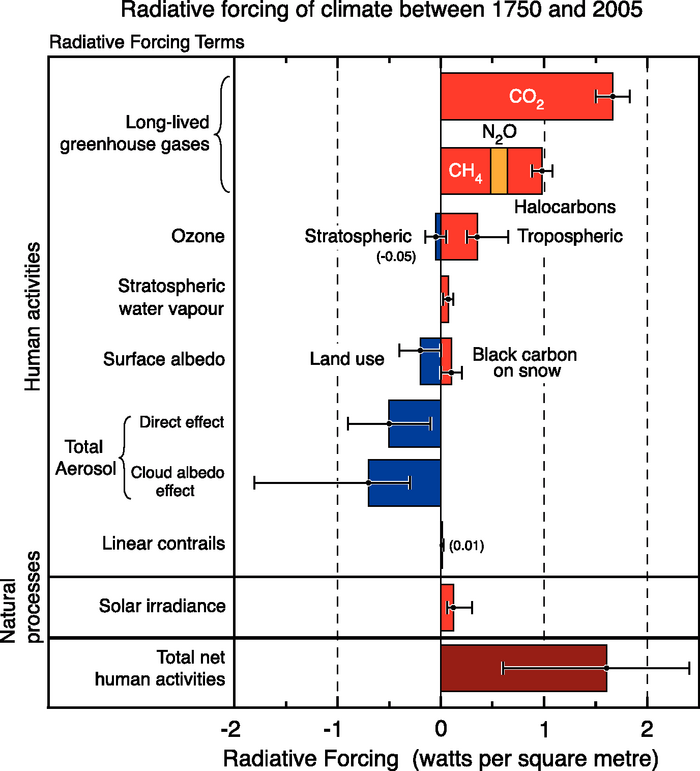
\includegraphics[width=\textwidth]{Figures/IPCC_WG1AR4_RFSummary.png}
      \caption{%
        The overall radiative forcings and uncertainties of several atmospheric constituents
        This is an image taken from \cite{IPCC_Chapter2}, found at \url{https://www.ipcc.ch/publications_and_data/ar4/wg1/en/faq-2-1.html}.}
      \label{LR:VOCs:IsopCascade:SOA:fig_IPCC_RF_AR4}
    \end{figure}
    
    \begin{figure}
      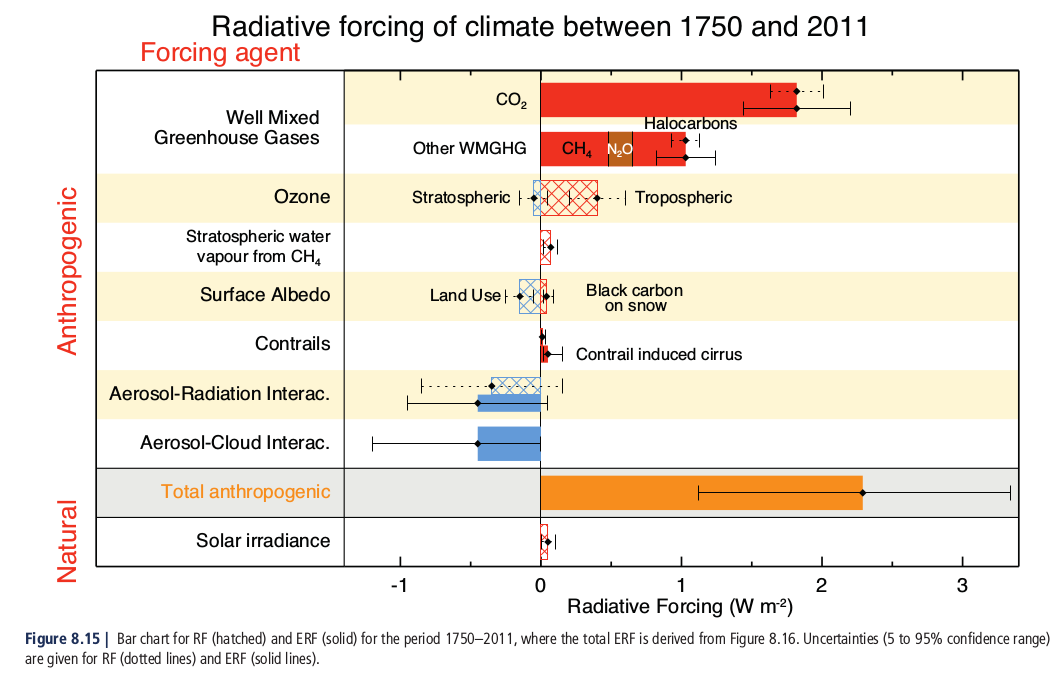
\includegraphics[width=\textwidth]{Figures/IPCC_WG1AR5_RFSummary.png}
      \caption{%
        The overall radiative forcings and uncertainties of several atmospheric constituents
        This is an image taken from \cite{IPCC_AR5_WG1}, chapter 8.}
      \label{LR:VOCs:IsopCascade:SOA:fig_IPCC_RF_AR5}
    \end{figure}    
    
    \cite{Kanakidou2005} highlight the need for improving emissions and flux measurements, in addition to utilising satellite data in models as a means of improving the emissions inventories.
    Observed nucleation outside of laboratories can arise from biogenic SOAs, driven by ozonolysis.
    \cite{Kanakidou2005} concluded that it is very likely that organics contribute to particle growth and formation rates.
    
\section{HCHO}
\label{LR:HCHO}
  
  % Lead in for HCHO section
  One of the major products of isoprene chemistry is HCHO.
  HCHO is important both for its own sake, and as a proxy for determination of isoprene emissions.
  Using the estimated yield of HCHO from precursor emissions allows us to estimate these precursors.
  
  % What is HCHO:
  HCHO, aka methanal, methyl aldehyde, or methylene oxide, is of the aldehyde family.
  HCHO is an OVOC which is toxic, allergenic, and a potential carcinogen. 
  It is dangerous at low levels, with WHO guidelines for prolonged exposure at 80~ppb.
  HCHO is used as an adhesive in plywood, carpeting, and in the creation of paints and wallpapers.
  Emissions in enclosed spaces can build up to dangerous levels, especially if new furnishings are installed (\cite{Davenport2015}).
  At global scales HCHO in furniture is less important, as concentrations are driven by photochemical reactions with methane and other VOCs.
  
  \subsection{Sources and sinks}
    \label{LR:HCHO:Sources}
     
    %Background hcho
    Background levels of HCHO in the atmosphere are driven by the oxidation of methane (CH$_4$) by the hydroxyl radical (OH$^{-1}$).
    \cite{Atkinson2000} summarised the background formation of HCHO with the following reaction:
    \begin{equation*} \label{LR:HCHO:Sources:eqn_MethaneBackground}
      OH + CH_4 (+ h\nu) + 2NO + 2O_2 \rightarrow OH + HCHO + H_2O + 2O_3
    \end{equation*}
    which shows that photolysis and oxidation of methane forms HCHO and ozone in a process that regenerates the OH radicals.
    CH$_4$ concentrations are thought to be well constrained in models, with the ACCMIP comparison showing only $\sim3$\% inter-quartile range (\cite{Young2013}).
    There is a complex relationship between VOCs, HO$_X$, and NO$_X$, and with higher levels of NO$_X$ the speed that VOCs are converted into HCHO increases, as does the HCHO concentration (\cite{Wolfe2016}).
    
    %cbl hcho
    Within the continental boundary layer, the major source of HCHO enhancement is VOC emissions reacting with OH radicals in the presence of NO$_X$ (\cite{Wagner2002, Millet2006, Kefauver2014}).
    Enhancements to regional and continental HCHO are largely driven by isoprene emissions (\cite{Guenther1995, Palmer2003, Shim2005, Kefauver2014}).
    This is true except near fires or anthropogenic sources of HCHO and precursors (\cite{Guenther1995, Kefauver2014, Wolfe2016}).
    Biomass burning (BB) can be a source of HCHO, and various other pollutants, precursors, and aerosols (\cite{Guenther1995, Andreae2001}).
    Additionally HCHO is emitted into the atmosphere directly through fossil fuel combustion, natural gas flaring, ethanol refining, and agricultural activity (\cite{Wolfe2016}).
    
    Other terpenoids (monoterpenes, sesquiterpenes, etc.) can also produce HCHO, although generally to a lesser extent than isoprene, methane and biomass burning (\cite{Guenther2012}).
    Many of the HCHO yields from terpenoids are estimated through chamber studies which examine the products molecular mass and charge after mixing the compound of choice into a known volume of air (\cite[eg.]{Nguyen2014}).
    These conditions generally don't match those of the real world, where ambient air will have a cocktail of these compounds as well as various reactants.
    \cite{Nguyen2014} state that one of their goals is to recreate ambient atmosphere in their chamber studies with more accuracy, in order to improve interpretations and allow more accurate model parameters.
    
    %Anthro Sources
    \cite{Millet2008} show that anthropogenic emissions of HCHO in America are mostly negligible, although improved sensitivity from oversampling allowed satellite detection of enhanced HCHO concentrations over Houston and Texas \citep{Zhu2014}.
    This is not the case in China, since massive population centres and industrial districts are emitting huge amounts of VOCs into the atmosphere \citep{Fu2007}.
    \cite{Fu2007} use GOME measurements over Asia and derive biogenic, anthropogenic, and pyrogenic VOC emissions, and \cite{Zhu2014} use oversampling of the OMI HCHO measurements to determine anthropogenic highly-reactive VOC emissions.
    Then with their updated emissions they show how surface ozone is affected, with a seasonal increase of 5-20~ppb simulated by GEOS-Chem.
    
    In the past, HCHO levels were underestimated by models, often with large discrepancies, due to the poor understanding of methyl peroxy radical (CH$_3$OO) chemistry (\cite{Wagner2002}).
    Nowadays HCHO concentrations are better understood, however precursor emissions are one of the main unknowns (\cite[eg.]{Emmerson2016,Marvin2017}).
    \cite{Marvin2017} found that discrepancies in modelled HCHO concentrations are primarily due to second and later generation isoprene oxidation chemistry.
    
    %% HCHO SINKS
    HCHO has two major sinks, one being reactions with OH (oxidation), the other being photolysis: the process of being broken apart by photons (\cite{Crutzen1999, Wagner2002, Levy1972, Kefauver2014}).
    These reactions lead to a daytime lifetime of a few hours (\cite{Atkinson2000, Millet2006}).
    Both these loss processes (photolysis, oxidation) form CO and hydroperoxyl radicals (HO$_2$), and have global significance to radiative forcing and oxidative capacity (\cite{Franco2015}).
    The other notable sinks are wet and dry deposition, although these are not as significant (\cite{Atkinson2000}) (TODO: add more cites here).
    
  % How measured (in-situ, satellite)
  \subsection{Measurement techniques}
  \label{LR:HCHO:Measurements}
    % how to measure HCHO
    There are a few ways to measure HCHO, including Fourier Transform Infra-Red Spectrometry (FTIR) and Differential Optical Absorption Spectroscopy (DOAS).
    FTIR examines the Fourier transform of a measured spectrum in order to determine what trace gases are interfering within the IR range of light.
    DOAS methods are based on light interference and absorption through air masses.
    
    The DOAS technique takes advantage of the optically thin nature of HCHO in order to linearise the radiance differential through air masses with and without HCHO, using the Beer-Lambert intensity law.
    This method works for both in the home HCHO detection and global measurements from in-situ and remote sensing instruments (\cite{Guenther1995, Abad2015, Davenport2015}).
    As a trace gas HCHO interferes with light over a few wavelength bands, which allows instruments to detect concentrations between a known light source and a detector.
    Figure \ref{LR:HCHO:Measurements:fig_HCHOSpectrum} shows the interference spectrum of HCHO as well as a typical band used to examine interference in the DOAS technique.
    One difficulty is that this interference is relatively small (HCHO is optically thin) and other compounds absorb light at similar wavelengths (\cite{Davenport2015}).
    
    \begin{figure}
      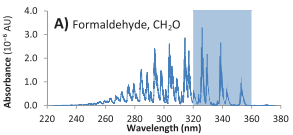
\includegraphics{Figures/HCHO/HCHOAbsorbanceDavenport.png}
      \caption{ %
        HCHO spectrum, with a typical band of wavelengths used for DOAS path measurements.
        This is a portion of an image from \cite{Davenport2015}.}
      \label{LR:HCHO:Measurements:fig_HCHOSpectrum}
    \end{figure}
    
    FTIR measurements can have a range of uncertainties, including systematic and random measurement errors and uncertain apriori shape factors and water profiles (eg: \cite{Franco2015}).
    Other types of measurement involve directly measuring the air, and determining chemical compounds through their physical properties.
    A proton transfer reaction mass spectrometer (PTR-MS) can be used to determine gas phase evolution of terpene oxidation products (\cite[eg.]{Lee2006a,Nguyen2014,Wolfe2016}).
    This is done through analysis of mass to charge ratios ($m/z$) of ionised air masses which are then identified as chemical compounds.
    \cite{Nguyen2014} use and compare several instruments (including one which is PTR-MS based) in the analysis of isoprene and monoterpene products.
    A Gas Chromatography mass spectrometer (GC-MS) is also able to identify isoprene, monoterpenes, and their products \cite[eg.]{Nguyen2014}.
    % TODO: Explain and find a couple of chamber studies to cite (should already be in my thing)
    
    Other measurement techniques include chromatographic and fluorimetric methods, both of which differ widely from each other and the spectroscopic methods (\cite{Hak2005}).
    \cite{Hak2005} examine a single air mass with 8 instruments using the four techniques (MAX-DOAS, FTIR, chromatographic, and flourimetric), and show that reasonable agreements can be achieved.
    Generally the measurements were somewhat close, the five Hantzsch instruments agreeing to within 11\% (after removing two potentially faulty measurements), although different calibration standards were used.
    Titration for the different calibration solutions could not be resolved, which may account for absolute offsets up to 30\%.
    These differences and non-uniformities between measurements (even among identical instruments) are part of the reason HCHO does not have a consistent network for global measurements like those for GHGs or Ozone (\cite{FortemsCheiney2012}).
  
    
  
  \subsubsection{Satellite measurements}
  \label{LR:HCHO:Sat}
    
    Several satellites provide long term trace gas observations with near complete global coverage, including the ERS-2 launched in April 1995 which houses the GOME ultraviolet and visible (UV-Vis) spectrometer, the AURA launched in July 2004 which houses the OMI UV-Vis spectrometer, the MetOp-A and B launched in October 2006 and September 2012 respectively both housing a GOME-2 UV-Vis spectrometer.
    These satellites are on Low Earth Orbit (LEO) trajectories and overpass any area up to once per day.
    Satellites can use DOAS techniques with radiative transfer calculations on solar radiation absorption spectra to measure column HCHO .
    An example of a spectrum retrieved from the GOME-2 instrument is given in figure \ref{LR:HCHO:Sat:fig_GOME_products}.
    
    \begin{figure}
      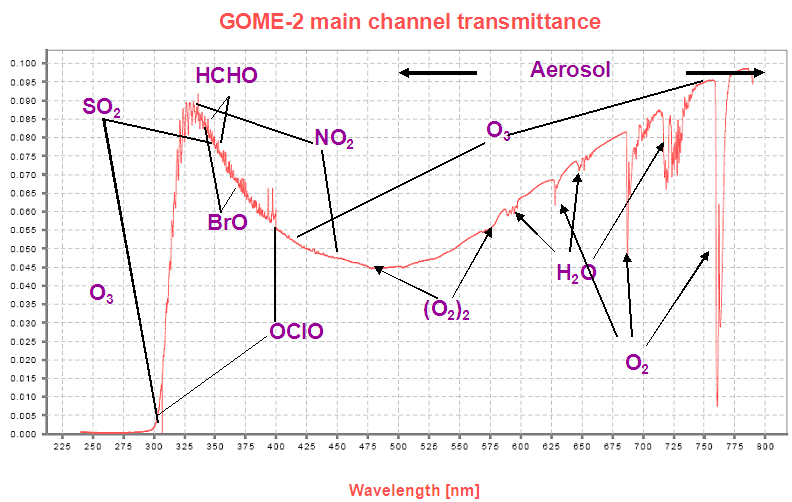
\includegraphics[width=\textwidth]{Figures/GOME_SPECTRUM.jpg}
      \caption{%
        An example spectrum showing interferences used for species concentration measurements by GOME-2. Image by EUMETSAT and ESA (\cite{GOME2Image}).
        }
      \label{LR:HCHO:Sat:fig_GOME_products}
    \end{figure}
    
    % Lead in to modelling
    In conjunction with atmospheric chemistry and radiative models, satellite measurements can be used to quantify the abundance of several chemical species in the atmosphere.
    Isoprene is hard to measure directly due to its short lifetime and weak spectral absorption, instead HCHO is often used as a proxy (\cite{Millet2006, Fu2007, Dufour2009, Marais2012, bauwens2013satellite, Kefauver2014, Bauwens2016}).
    This leads to a method of isoprene emissions estimation termed top-down (as opposed to bottom-up estimates like MEGAN).
    The existence of satellite data covering remote areas provides an opportunity to improve VOC emissions estimates leading to more robust models of global climate and chemistry. 
    Satellite data allows us to verify large scale models of natural emissions, and their subsequent chemistry.
  

  
\section{Atmospheric Chemistry Modelling}
\label{LR:Models}
  
  Models can fill the gaps (both spatial and temporal) in measurement records, and are used to predict/prevent/understand various scenarios.
  They are used ideally to steer us away from unsustainable pollution and help complete our understanding of the world from small to large scales.
  They can be used to increase measurement accuracy (for instance in satellite measurements) and determine where we lack information, while also checking the performance of new instruments.
  Precisely representing various chemicals and reactions in the atmosphere allows efficient mitigation of pollution, since we can compare scenarios against one another.
  Currently, improved isoprene understanding is critical for effective air quality measuring \citep{Marvin2017}.
  
  Atmospheric chemical models provide a simulation of chemical densities and transport over time, through the atmosphere.
  They require various inputs in order to accurately represent scenarios or regions on earth.
  Models of emissions are often used as drivers for atmospheric chemistry models, which generally require initial and boundary conditions in order to run.
  The chemistry in the atmosphere is a complex system of coupled reactions and dynamics, and is generally solved using numerical partial differential equation solvers.
  
  Chemical Transport Models (CTMs) simulate production, loss, and transport of chemical species.
  This is generally calculated using one or both of the Eulerian (box) or Lagrangian (puff) frames of reference.
  CTMs normally solve the continuity equations simultaneously with chemical production and loss for chemicals under inspection.
  The continuity equations describe transport of a conserved quantity such as mass, which, solved together with production and loss of a chemical can provide detailed simulations of natural processes.
  
  The general continuity equation links a quantity of a substance (q) to the field in which it flows and can be described by the formula:
  \begin{align*}
    \frac{\partial \rho}{\partial t} + \nabla \cdot j &=& \sigma 
  \end{align*}
  where $\rho$ is density of q in the field, t is time, $\nabla$ is divergence, j is the flux (q per unit area per unit time entering or leaving the field), and $\sigma$ is the generation or loss of q per unit volume per unit time.
  
  
  The type of model best suited to modelling the entire earth uses the Eulerian frame of reference, where the atmosphere is broken up into 3-D boxes with densities and transport calculated and stored for sequential steps in time at each location.
  The mass balance equation must be satisfied in any realistic long term box model and is as follows: 
  \begin{align*}
    \frac{dm}{dt} &=& \sum{sources}-\sum{sinks} \\
    &=& F_{in} + E + P - F_{out} - L - D 
  \end{align*}
  where m is mass of a chemical, E and D are emission and deposition, P and L are production and loss, and F is chemical transport in and out, as shown in figure \ref{LR:Models:fig_boxmodel}.
  Many chemical species interact with each other through production and loss. 
  Any large chemical model will solve this mass balance equation over highly coupled arrays of partial differential equations which can be complex and time consuming.
  
  \begin{figure}
    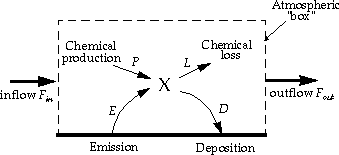
\includegraphics{Figures/boxmodel.png}
    \caption{ %
      Standard box model parameters, image taken from \cite{Jacob_1999_book}. }
    \label{LR:Models:fig_boxmodel}
  \end{figure}
  
  
  Contemporary models generally use mathematical differential solving tools of various complexity to solve chemical equations and reaction rates (often called chemical mechanisms) in order to predict an environments evolution over time.
  Different solvers may be slower or faster and more suited to particular situations based on the stability of the equations and systems involved, and chemical mechanisms may vary in how many reactions and chemicals are listed and grouped together.
  For example: Since [O] $<<$ [O$_3$] the chemical family O$_X$ (  O$_X \equiv $ O $+$ O$_3$ ) can be used to simplify chemistry simulations and approximate O$_3$ concentrations \citep[][Chapter 3]{BrasseurJacob2017}.
  \cite{Zhang2012} examine the outputs from a regional model (WRF/Chem) using three different chemical mechanisms, and they show that particulate matter prediction is sensitive to the choice of chemical mechanism. 
  
  
  \subsection{Box models}
    Box models are much smaller scale than global CTMs, examining one uniform environment with many parametrisations such as transport and emissions.
    Box models can be used to check chemical mechanisms in specific scenarios, such as high or low NO$_X$ environments.
    \cite{Marvin2017} use a box model matching conditions in southeast USA to evaluate isoprene mechanisms from several models.  
    A box model involves modelling chemistry in a singular set of conditions without transport or any spatial gradients.
    One box model used in this thesis is called CAABA/MECCA, and is described in Section \ref{Model:CM}.
    
    By allowing for interactions between boxes this concept can be extended to multiple-box models.
    These are simply multiple instances of single boxes with the addition of transport between them, which generally requires a meteorological model to provide winds, and other transport mechanisms.
  
  
  \subsection{Emissions}
  
    %% HOW estimates are made
    There are two commonly used ways of estimating isoprene emissions, top-down or bottom-up.
    Bottom-up emission estimates generally model the flora and events which emit isoprene, like Eucalypts, factories, shrubs, etc.
    They use various properties of the emitters in order to estimate how much isoprene is being produced.
    Some of these properties include leaf areas, speciated responses to sunlight and temperature, moisture stress, etc (\cite{Guenther1995,Guenther2006}).
    Understanding how much isoprene is emitted, when and by what, is complicated.
    Since little data exists with which to verify many of these bottom-up emission inventories, they can be uncertain on a large scale.
    Emissions inventories such as MEGAN are bottom-up and use models of emissions based on tree types, weather, and other parameters.
    
    In many CTMs the isoprene emissions are calculated seperately (for example by running MEGAN), and then used as boundary conditions (EG: \cite{Guenther2006}). 
    This can speed up calculations as the transport and concentrations can be simulated in various conditions without recalculating the emissions.
    Trace gases with short lifetimes and complex chemistry such as isoprene are often hard to measure which makes verifying model estimates difficult.
    
    Bottom up models of VOC emissions are sensitive to parameters.
    \cite{Stavrakou2014} examined modelled Asian emissions and altered model parameters for temperature, plant type emission factors, incoming solar radiation (insolation) intensity, land use changes, and palm tree forest expansion.
    Changes were constrained by a network of radiation measurements and some experiments with south east Asian forest emissions - and led to reduction in isoprene emissions by a factor of two over the region.
    The Asian region is shown to have a strong correlation with the Oceanic Ni$\tilde{n}$o Index (ONI), with positive anomalies associated with El Ni$\tilde{n}$o.
    
    
    \cite{Marais2014} examine factors affecting isoprene emissions, showing how emissions are sensitive to various environmental factors.
    Their work used MEGAN \citep{Guenther1995} and GEOS-Chem to look at how these factors affect surface ozone and particulate matter in Africa.
    One of the important uncertainties seen in MEGAN within this work is the isoprene emissions due to plant type.
    Canopy level isoprene measurements are made using relaxed eddy accumulation (REA) at several sites in Africa.
    One plant type near a measurement site emits more than other species and it's actual distribution on a larger scale is completely unknown - leading to possible overestimations in MEGAN.
    Current emissions estimates require more validation against observations, and recently a comparison of two major VOC models (MEGAN and ORCHIDEE) was undertaken by \cite{Messina2016} reiterating this requirement.
    In their work they examine model sensitivities and show that the important parameters are leaf area index (LAI), emission factors (EF), plant functional type (PFT), and light density fraction (LDF).
    There is high uncertainty in LAI and EF, which require more or improved measurements at the global scale.
    LDF paramterisation needs improvement and these models require more PFTs.
    Global emissions inventories like MEGAN suffer from large extrapolations which introduce uncertainties \citep{Miller2014}.
  
  
  \subsection{Uncertainties?}
  \label{LR:Models:Uncert}
    
    Here I will attempt to list and partially explain the major uncertainties models have in relation to  VOCs, SOAs, and ozone. 
    TODO: Is this a good idea or should I put any pertinent uncertainties with the associated work/descriptions?
    
    
    \subsubsection{Emissions Inventories}
      % Emissions Inventories 
      Using different emissions inventories in an ACM can have large impacts on the simulation.
      Natural (biogenic or pyrogenic) and human driven (anthropogenic) emissions often drive a large fraction of atmospheric oxidation and radical chemistry, especially in the continental boundary layer.
      \cite{Zeng2015} examine the affects on CO and HCHO when running simulations with two different inventories.
      TODO: find where I took notes about Zeng2015 and put them here.
      
      It is important to note that many estimates of isoprene emission are based on a few algorithms which can depend greatly on input parameters (\cite{Arneth2008,Niinemets2010}).
      \cite{Arneth2008} argue that this monopoly of emissions estimates may be leading us to an incorrect understanding of isoprene chemistry.
      \cite{Yue2015} has shown that this is still a problem by looking at land carbon fluxes and modelling the sensitivity to VOC emissions estimates using two independent models of VOC emission.
      One model is photosynthesis based and estimates isoprene emissions using electron transfer energies and leaf physiology \citep{Niinemets1999}, while the other (MEGAN) uses the light and canopy temperature (\citep{Guenther1995,Arneth2007} TODO: Read Arneth et al., 2007; Unger et al., 2013).
      Both are sensitive to light and temperature parameterisations.
      
      % Uncertainties in estimates
      Isoprene emissions estimates are still fairly uncertain, as global measurements are difficult and regional emissions can be very different. 
      %In 2005, Dr. C. Wiedinmyer et al. reviewed emissions inventories and showed %TODO 
      The global uncertainty of isoprene emission was estimated to be a factor of 2 to 5 (250-750\tgpyr) \citep{Kanakidou2005}.
      Improvements over the years have been incremental, and generally localised to regions of particular interest for air quality such as China and the USA TODO: find recent uncertainty estimate improvements examples.
      The lack of accuracy in BVOC emissions estimates prevents accurate determinations of the sources and distribution of pollutants including ozone and organic aerosols.
      Most of the tropospheric SOA comes from biogenic precursors, the evidence for this has grown over the last two decades \citep{Guenther1995, Kanakidou2005,Guenther2012}.
      Accuracy in VOC measurements is important: it has been shown that even the diurnal pattern of isoprene emissions has an effect on modelling ground level ozone \citep{Hewitt2011, Fan2004}.
      
      Improvements to emissions models require improved understanding of regions and their behaviour.
      Inaccuracies can arise due to lack of data, such as the large and sparsely measured Australian outback.
      MEGAN has been shown to overpredict isoprene and underpredict monoterpene emissions in southeast Australia, with peaks and troughs captured but not at the right magnitude (\cite{Emmerson2016}).
      MEGAN output in Australia is adversely affected by poor emission factor estimation. 
      An example can be seen in \citet{Muller2008} where MEGAN overestimates isoprene in northern Australia.
      Underestimates of monoterpenes may be due simply to underestimated emission rates for many Eucalypt species \citep{Winters2009}.
    
    %% GEOS-Chem resolution uncertainties
    \subsubsection{Resolution}
      \label{LR:Models:Uncert:Resolution}
      GEOS-Chem simulations are somewhat sensitive to the resolution at which you run.
      For example: \cite{Wild2006} show that reduced resolution increases OH concentrations and ozone production rates.
      \cite{Christian2017} find small changes in OH ($<10$\%) in OH, HO$_2$ and ozone concentrations local to the north american arctic, when changing from 4 by 5 to 2 by 2.5\degr resolution, however they continue at lower resolution to save computational time.
    
      For many global scale analyses, errors from resolution are less important than those from chemistry, meteorology, and emissions (\cite{Christian2017}).
      Many models lack in-situ measurements with which to verify their chemical mechanisms, leading to large discrepancies, as seen in \cite{Marvin2017a}.
      TODO: briefly talk about Marvin2017a takeaways.
      \cite{Christian2017} used GEOS-Chem v9-02, with $4^{\circ} \times 5^{\circ}$ resolution, and while the low resolution adds errors in OH concentrations and O$_3$ production rates, the errors from chemistry, meteorology, and emissions are much larger.
            
    
    \subsubsection{Chemistry mechanisms}
      \label{LR:Models:Uncert:Chemistry}
      %% GEOS-Chem Ozone uncertainties 
      There is still much work to be done in models to correctly simulate the various precursors to HCHO.
      Often HCHO is used as a way of checking if these precursors are correctly modelled since HCHO measurements are more readily available (for instance from satellites).
      GEOS-Chem has recently been analysed for sensitivity for ozone along with oxidants (OH and HO$_2$) \citep{Christian2017}.
      \cite{Christian2017} found that GEOS-Chem ozone was most sensitive to NO$_2$ photolysis, the $NO_2 + OH$ reaction rate, and various emissions.

      \cite{Marvin2017} suggest that isoprene mechanisms in several contemporary models (including GEOS-Chem) are inadequate. 
      They show that for a specific measurement campaign, the HCHO concentrations are underestimated in a way that can not be easily fixed through rate constant changes.
      Recently \cite{Marvin2017} compared five global ACMs isoprene mechanisms by evaluating simulated HCHO mixing ratios compared to in situ measurements from the Southeast Nexus (SENEX) aircraft campaign (in southeastern USA).
      They compared five models (GEOS-Chem, CB05, CB6r2, MCMv3.2, and MCMv3.3.1) and found all of them underestimated the HCHO concentrations (by $15 - 30\%$).
      
      Another important factor in determining the yield of HCHO and other products from BVOCs is the local concentration of NO$_X$.
      \cite{Travis2016} show how modelled surface ozone is overestimated due to high estimates of  NO$_X$ emissions, which affect oxidative capacity and VOC reactions.
      
    
    \subsubsection{Clouds}
      \label{LR:Models:Uncert:Clouds}
      One of the major uncertainties in chemical, climate, radiation, and weather models is cloud formation and dynamics.
      Clouds are remarkably complex at a much finer scale than can be accurately modelled by global chemistry models (with current processing power).
      Globally over half (50-60\%) of the world is covered by clouds, with $\sim10\%$ of them being rain-clouds \citep{Kanakidou2005}.
      Wet scavenging performed in clouds not only depends on large scale cloud processes, but also on the microphysics of aerosols being scavenged, differing between aerosol sizes and hygroscopic properties.
      
    
    \subsubsection{Soil Moisture}
      \label{LR:Models:Uncert:SoilMoisture}
      Australia has a unique climate, along with soil moisture, clay content and other important properties which affect VOC emissions.
      These properties are poorly understood in Australia due to the continents size and the relative sparsity of population centres, which make many areas very difficult or expensive to reach.
      \cite{Rowntree1983} show how quickly soil moisture anomalies affect rainfall and other weather systems, while \cite{Chen2001} specifically show how important fine scale soil moisture information is when modelling land surface heat flux, and energy balances.
      Modelled emissions are sensitive to soil moisture, especially near the soil moisture threshold (or wilting point), below which trees stop emitting isoprene and other VOCs completely as they can no longer draw water \citep{Bauwens2016}.
      MEGAN accounts for soil moisture by applying it as an emission factor (EF) which scales the emission rate of various species.
      
      
      Droughts affects can be difficult to measure, as it is a multi-scale problem which affects various aspects of the land-air interface including plant emissions and dry deposition (\cite{Wang2017}).
      The Standardised Precipitation Evapotranspiration Index (SPEI) is a measure of drought using TODO \cite{SPEI_website}.
      This product covers 1901 - 2011, and uses the average over that period as the background, in order to compare drought stressed regions against those with sufficient or excess water \cite{SPEI_website}.
      
    
    
  
\section{Australia and the southern hemisphere}
\label{LR:Aus}
  % Description of uniqueness
  In Australia most long term air quality or composition measurements are performed in or near large cities.
  Australia is dominated by areas with little anthropogenic influence and no ground based measurements of the natural emissions taking place \citep{VanDerA2008}.
  Due to the lack of in-situ ground based measurements, estimates of VOC emissions are uncertain, with large scale extrapolation required \cite{Millet2006}.
  Since many Australian cities are on the edge of regions with rich VOC emissions, it is very important to clarify the quantity, type, and cause of VOC emissions.
  Understanding of emissions from these areas is necessary to inform national policy on air pollution levels.
  
  
  %Transport stuff
  Fire emissions include a range of chemicals and each year the affects of fire or burning seasons blanket the northern and southern hemispheres independently.
  Biomass burning in southern Africa and South America has previously been shown to have a major influence on atmospheric composition in Australia \citep{Oltmans2001, Gloudemans2006, Edwards2006}, particularly from July to December \citep{Pak2003, Liu2016}.
  
  % More uniqueness
  \cite{Guenther2006} estimated that the Australian outback is among the worlds strongest isoprene emitters with forests in SE Australia having emission factors greater than 16 mg m$^{-2}$ h$^{-1}$ (see figure \ref{LR:Aus:fig_MEGAN_EF}).
  Measurement campaigns in SE Australia have since cast doubt on the emission factors used by MEGAN, as the Eucalyptus trees and soil moisture were poorly studied \cite{Emmerson2016}.
  These emissions factor estimates are not well verified and measurements of isoprene (or other BVOC) emissions barely cover Australia either spatially or temporally.
  However, comprehensive coverage of one high yield product (HCHO) in the atmosphere over Australia exists in the form of satellite measurements.
  
  \begin{figure}
    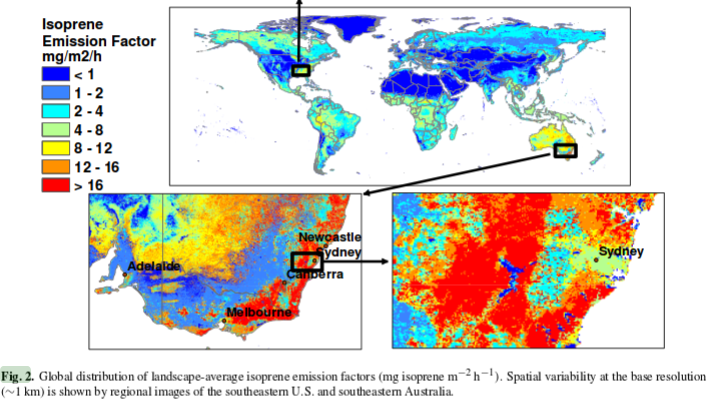
\includegraphics[width=\textwidth]{Figures/MeganIsoprene1.png}
    \caption{ Part of a figure from \cite{Guenther2006} showing global isoprene emission factors. }
    \label{LR:Aus:fig_MEGAN_EF}
  \end{figure}
  
  
  \subsection{Ozone}
    Ozone levels over Australia are generally low, however it remains unclear how much we would expect this to change in the future as relatively little is known about precursors and influx for the continent.
    % Air Quality metric example
    Australian air quality is monitored independently within each state, using various metrics. These metrics are measured by varying numbers of monitoring stations in each state.
    In New South Wales (NSW) the metrics used to determine air quality are: particulate matter (PM), O$_3$, CO, NO$_2$, SO$_2$, and visibility.
    An air quality index equal to the worst of these metrics is used for NSW as shown at \url{http://www.environment.nsw.gov.au/aqms/aqitable.htm}.
    Similar methods are used in other states to get an idea of air quality.
    Measurement stations are generally located in population centres, and don't regularly measure precursor emissions. 
    This is an important omission as naturally emitted precursor gases often get transported into cities where they affect air quality through production of O$_3$ and other pollutants.
    
    Generally STT over australia affects the upper troposphere only, however ozone enhancements can reach quite low during heavy storms and cyclonic weather patterns (\cite{Alexander2013})
  
  % voc estimates
  \subsection{VOCs}
    Bottom up inventories of VOCs remain largely uncertain due to extensive extrapolation over plant functional types, changing land cover, and parameterised environmental stressors \citep{Guenther2000,Kanakidou2005,Millet2006}.
    VOC emission estimates are highly sensitive to many factors, several of which are not well characterised in Australia \citep{Sindelarova2014, Bauwens2016}.
    Changes in parameterisation of soil moisture in the Model of Emissions of Gases and Aerosols from Nature (MEGAN, \cite{Guenther1995}) lead to massive changes in Australian isoprene emission estimates \citep{Sindelarova2014}.
    Over Australia MEGAN has problems involving unpublished plant functional types and their emissions, as well as poorly optimised soil moisture parameterisation \citep{Emmerson2016}.
    
    Australia has the potential to be a major hotspot of isoprene emissions according to \cite{Guenther2006,Guenther2012}, which shows heavy emissions factors in the region.
    Although recent work suggests that some Australian eucalypts may not be as egregious isoprene emitters as once thought \cite{Emmerson2016}.
    Emissions in MEGAN are based on plant functional types, which can vary heavily even within species.
    TODO: more on Muller2008
    Australia also lacks a clear estimate of emitted monoterpenes.
    
    \cite{Emmerson2016} analyse EF sensitivity of a high resolution model of atmospheric chemistry over southeast Australia, comparing isoprene and monoterpene emissions against 4 separate campaigns.
    They show that the effect on total emissions is roughly linear and that no blanket EF changes are appropriate for all regions/seasons.
    They also mention that Australian eucalypt emissions are based on samples from young trees, which may emit more isoprene than older trees.
    \cite{Emmerson2016} suggest that monoterpenes may be emitted in similar quantites to isoprene, with more measurements required to determine if this is so.
    They compare emissions estimates from MEGAN against data from several field campaigns and see overestimated isoprene emissions, as well as underestimated monoterpene emissions.
    Their work suggests that MEGAN estimates of isoprene emissions may be 2-6 times too high, and monoterpene emissions $\sim3$ times too low over southeast Australia.
    
    This problem is even more pronounced in Australia due to poor characterisation, or because emission factors are based on northern hemispheric data.
    Many plant emissions rates have not been published, such as those for any Australian acacias.
    Additionally soil moisture is not well quantified which has a large effect on emissions.
    \cite{Muller2008} show how isoprene is poorly captured by the MEGAN model and analyse the affect of changing the soil moisture parameter, which can reduce the overall bias for Australia.
    \cite{Sindelarova2014} show reductions in modelled Australian isoprene emissions of 50\% when incorporating soil moisture in MEGAN estimates. 
    Uncertainties in isoprene emissions could explain why models of HCHO over Australia are poor at reproducing satellite measurements \citep{Stavrakou2009}.
    
  
  
  \subsection{Measurements}
    
    % TODO: Campaigns
    TODO: Brief overview of all the measurement campaigns, pointing to Modelling and Data chapter for more details.
    There are relatively few measurements of isoprene in the southern hemisphere, including MUMBA(TODO CITE), other campaigns?, and very recently that girl from Macquarie University with an instrument in the daintree rainforest(TODO CITE, DESCRIBE?).
    For details on the MUMBA campaign see Section \ref{Model:Datasets:MUMBA}.
    An airflight campaign (HIPPO) measuring isoprene was also performed in 2009-2011? TODO: ask Jenny re this one.
    
    A particulate and air quality measurement campaign took place in Sydney using PTR-MS and GC-FID, for details see Section \ref{Model:Datasets:SPS}.
    
    One method of measuring ozone in the troposphere and stratosphere is by releasing weather balloons (with attached ozone detectors) which take readings as they rise up to around 30~km, giving a vertical profile of concentrations.
    Since 1986, Lauder, New Zealand (45$^{\circ}$S, 170$^{\circ}$E) has released ozonesondes allowing a multi-decadal analysis of ozone concentrations over the city \citep{Brinksma2002}.
    Kerguelan Island (49.2$^{\circ}$S, 70.1$^{\circ}$E), also has a record of ozonesonde profiles, which are directly in the path of biomass burning smoke plumes transported off shore from Africa \citep{Baray2012}.
    SHADOZ is the southern hemispheric additional ozone project, which have released sondes from 15 sites at different times \url{http://tropo.gsfc.nasa.gov/shadoz/}.
  
\section{Aims}
\label{LR:Aims}
TODO: outline of aims here (FIND THESE THEY ARE SOMEWHERE)
  
  \textbf{One of the aims in this thesis is to use the available satellite measurements to improve the estimates of isoprene emissions in Australia.}
  Satellites which overpass daily record reflected solar (and emitted terrestrial) radiation, and give us measurements over all of Australia.
  Combining satellite data with model outcomes provides a platform for the understanding of natural processes which is especially useful over Australia.
  Due to the low availability of in-situ data over most of the Australian continent, a combination of the models with satellite can fill the gap of understanding of emissions from Australian landscapes.
  Improved emissions estimates will in turn improve the accuracy of CTMs, providing better predictions of atmospheric composition and its response to ongoing environmental change.
  
  Calculation of isoprene to HCHO yields over Australia is required to create top-down estimates.
  This requires among other things an idea of which VOCs are present and their yields of HCHO.
  The technique of determining isoprene emissions from satellite detected HCHO is called satellite inversion.
  \textbf{Another aim to this end is to run and become familiar with GEOS-Chem in order to determine Australian emissions and yields, and the importance of the relevant parameters.}
  Soil moisture plays an important role in VOC emissions, as trees under stress may stop emitting various chemicals. 
  This is especially true for Australia due to frequent droughts and wildfires.
  The argument for improved understanding of land surface properties, specifically soil moisture, is an old one\citep{Mintz1982, Rowntree1983, Chen2001}.
  
  \textbf{To improve understanding of ozone over the southern hemisphere including Australia.}
  Meteorology and precursor emissions are the largest drivers of tropospheric ozone concentrations, and an improved understanding of their effects in Australia would be facilitated by an analysis of STT as well as more confidence in the emitted precursors.
  
